\chapter{Prototyping}
%Development
Since no library with Android support currently exist it was decided to use the Motej library as a core for further development.

\section{Introduction}
At the time of writing no research has been done on using motion game controllers as peripherals in a smart-phone based bio-feedback system. In order to answer the research questions posed in this report it will be necessary to create a simple but working prototype of the aforementioned system. The equipment used to realize the system will be a rooted HTC Desire HD \cite{desireHdSpecs} running CyanogenMod 7 and Wii Remotes with the Motion Plus extension. The application will be created using the Android SDK, Java and the Motej library.
%Write about why we chose motej?

\section{Wii remote reverse engineering}
This section will look closer on the reverse engineering of the Wii remote. Since the Wii remote is the only sensor to be used in this project, it is important to explain in detail how the data from this sensor is parsed and calibrated. In this section there will be multiple references to Motea. Motea is a lightweight Wii remote API based on Motej \cite{Motej}, designed specially for this project. A further description of Motea can be found in section~\ref{sec:motea}

Nintendo has not released any documentation of how to connect to or use the Wii remote. All the information in this section is taken from internet communities \cite{wiiBrew} that have reverse engineered the Wii remote and from open source Wii remote API projects \cite{wiiMoteLib, Motej}.

The Wii remote is based on the HID protocol for communication, and will appear as such to any host. It is possible to connect to the Wii remote both with and without Bluetooth pairing. If paired the Wii remote will attempt to reconnect to the host if the connection is lost. In the current version Motea no pairing is performed. A HID connection is established using L2CAP, opening a data channel on port 0x13. This channel is used for both sending and receiving data.

\subsection{HID interface}
The different report types used in the Motea library are displayed in table~\ref{tab:hidInterface}. An output report represents a report that is sent from the host to the Wii remote. An input report is a report that is sent from the Wii remote to the host. Input reports are prefixed with 0xa1 and output reports are prefixed with 0xA2.There are more input reports than those listed in table~\ref{tab:hidInterface}, but they are not used by Motea since data report 0x35 contains all the data needed. 

\begin{table}[h!]
\centering
\begin{tabularx}{\textwidth}{|l|l|X|}
\hline
I/O & ID & Description \\ \hline
O & 0x11 & Set LEDs \\ \hline
O & 0x12 & Set data reporting mode \\ \hline
O & 0x15 & Request status information \\ \hline
O & 0x16 & Write to memory/registers \\ \hline
O & 0x17 & Read from memory/registers \\ \hline
I & 0x20 & Status information \\ \hline
I & 0x21 & Data from memory/register request \\ \hline
I & 0x35 & Data report containing data from core buttons, accelerometer and extension (gyroscope) \\ \hline
\end{tabularx}
\caption{\footnotesize The table describes the different output and input reports used by the application}
\label{tab:hidInterface}
\end{table}

\subsection{Output reports}
Motea sets the report mode to 0x35 as soon as the connection to the Wii remote is established. This is done by sending the following bytes to the Wii remote:
\begin{quote}
0xA2 0x12 0x04 0x35
\end{quote}
The first byte indicates that it is an output report, the second byte is the ID of the report type, the third byte indicates whether to use continuous reporting (send report even when there has been no change to the data) and the fourth indicates which report mode to set. The report mode has to be set again whenever an extension is discovered, this can be detected by the fact that you receive a status information report without requesting one. In such cases Motea immediately sends a request to set the report mode to 0x35.

Report mode 0x35 contains core button (0xbb), acceleromter (0xaa), and extension data (0xee):
\begin{quote}
0xA1 0x35 0xbb 0xbb 0xaa 0xaa 0xaa 0xee 0xee 0xee 0xee ... (16 bytes of type 0xee)
\end{quote}

The LEDs on the Wii remote can be controlled by using output report 0x11:
\begin{quote}
0xA2 0x11 0x80
\end{quote}
The third byte indicates which lights to turn on, the four most significant bits of this byte each represents one LED (in the example above the rightmost byte is enabled):
\begin{quote}
0b0000 0000 : no lights\\
0b1000 0000 : rightmost LED enabled\\
0b1100 0000 : the two rightmost LEDs enabled\\
etc.
\end{quote}
Motea also uses this report mode to initialize the rumble pack. The least significant bit of the third byte of any output report turns sets the status of the rumble pack, where 1 is on and 0 is off. As an example, let us say we have the two rightmost LEDs activated and the rumble pack is to be turned on, the report would look like this:
\begin{quote}	
0xA2 0x11 0xC1\\
(0xC1 = 0b1100 0001 the least significant bit representing the rumble pack)
\end{quote}
As previously stated all output reports have to change the least significant bit of the third byte to one if the rumble pack is to stay active. Therefore Motea has to keep track of the state of the rumble pack and change the output reports accordingly. All examples in this section, other than the one above, will assume that rumbling is turned off.

Status information can be requested by sending:
\begin{quote}
0xA2 0x15 0x00
\end{quote}
A status information report with ID 0x20 is then sent from the Wii remote to the host:
\begin{quote}
0xA1 0x20 0xbb 0xbb 0xss 0x00 0x00 0xll
\end{quote}
0xbb (bytes 3 and 4) contains data about the core buttons. 0xss contains data about which LEDs are enabled and whether the following features are enabled: speaker, extension controller, and continouous reporting. 0xll holds the battery level. 

Writing to registers is done by sending:
\begin{quote}
0xA2 0x16 0x04 0xaa 0xaa 0xaa 0xll 0xdd 0xdd ...
\end{quote}
Here 0xaa (bytes 4-6) represents the register address to write to. 0xll is the number of bytes to write. 0xdd (bytes 8-) is the data to be written to the register, usually only one byte is written.

Reading from registers/memory is done by sending:
\begin{quote}
0xA2 0x17 0xmm 0xaa 0xaa 0xaa 0xll 0xll
\end{quote}
0xmm sets whether to read from memory or from the registers, in motea only the calibration report for the accelerometer is read from memory. 0xaa (bytes 4-6) is the address to read from. 0xll (bytes 7 and 8) is the length of data to be read. After a read request is sendt the Wii remote sends the data in return using a report with ID 0x21:
\begin{quote}
0xA1 0x21 0xbb 0xbb 0xse 0xaa 0xaa 0xdd 0xdd ... (16 bytes of the type 0xdd)
\end{quote}
0xb (byte 3-4) is core button data. 0xse holds both the size of the data returned and the error flag. 0xdd (bytes 8-23) contain the requested data (as long as there was no error).

\subsection{Accelerometer}
Accelerometer data is received with every data report of ID 0x35:
\begin{quote}
0xA1 0x35 0xbb 0xbb 0xxx 0xyy 0xzz 0xee 0xee ...
\end{quote}
The accelerometer data each consists of 10 bits of x-axis data, and 9 bits of y- and z-axis data. Y- and z-axis data should also be represented as 10 bits, this is done by always letting the least significant bit be 0 for these axes (0bxx xxxx xxx0 where x is some data). The most significant bits of x-, y- and z-axis accelerometer data are located in 0xxx, 0xyy and 0xzz respectively. The least significant bits are located in he 0xbb bytes as shown in figure~\ref{fig:accelerometerData}, these bytes also contain core button data.
\begin{figure}[h!]
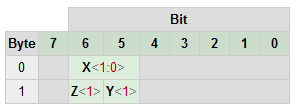
\includegraphics{accelerometerData.png}
\caption{\footnotesize Least significant bits of accelerometer data}
\label{fig:accelerometerData}
\end{figure}

In order to make sense of the accelerometer data they have to be calibrated. The calibration data is stored in the Wii remote and can be acquired by sending a read request:
\begin{quote}
0xA2 0x17 0x00 0x00 0x00 0x20 0x00 0x0a
\end{quote}

The Motej \cite{Motej} library did not contain any code for calibrating the acceleromter data. In Motea the calibration is based on an implementation found in the WiiMoteLib \cite{wiiMoteLib} library. Motea parsing and calibrating accelerometer data:
\begin{lstlisting}
// Get raw data
float x = 
	((bytes[4] & 0xff) << 2) | ((bytes[2] & 0xff) >> 5 & 0x03);
float y = 
	((bytes[5] & 0xff) << 2) | ((bytes[3] & 0xff) >> 5 & 0x02);
float z = 
	((bytes[6] & 0xff) << 2) | ((bytes[3] & 0xff) >> 5 & 0x02);

CalibrationDataReport c = source.getCalibrationDataReport();
if (c == null) {
	return;
}

// Calculate calibrated accelerometer data
x = (float) ((x - c.getZeroX()) / 
	(c.getGravityX() - c.getZeroX()));
y = (float) ((y - c.getZeroY()) / 
	(c.getGravityY() - c.getZeroY()));
z = (float) ((z - c.getZeroZ())	/ 
	(c.getGravityZ() - c.getZeroZ()));

source.fireAccelerometerEvent(x, y, z);
\end{lstlisting}

\subsection{MotionPlus}
\label{sec:gyroParse}
When you plug in a normal extension to the Wii remote it is automatically receive a status information report notifying that an extension has been connected. Pluging in the MotionPlus however, will not result in such a status information report. To check if the MotionPlus extension is pluged in, the two bytes from Wii remote register address 0xA600FE has to be read by sending the read request:
\begin{quote}
0xA2 0x17 0x04 0xA6 0x00 0xFE 0x00 0x02
\end{quote}
After sending this request a data report with ID 0x21 is sent in return containing the requested data. The received data report contains the two bytes read from register 0xA600FE. The meaning of these bytes are shown in table~\ref{tab:motionPlusStatus}. If the MotionPlus extension is not connected the data report will fail with error 7.
\begin{table}[h!]
\begin{tabularx}{\textwidth}{|l|X|}
\hline
Value  & Meaning \\ \hline
0x0005 & MotionPlus is pluged in, but not initialized \\ \hline
0x0405 & No longer active MotionPlus\\ 
\hline
\end{tabularx}
\caption{\footnotesize MotionPlus status}
\label{tab:motionPlusStatus}
\end{table}

After confirming that the MotionPlus extension is pluged in, the next thing to do is to initialize it. This is done by writing 0x55 to 0xA600F0, by sending the following report:
\begin{quote}
0xA2 0x16 0x04 0xA6 0x00 0xF0 0x01 0x55
\end{quote}

When the MotionPlus has been initialized it has to be activated before we can receive data from it. This is done by writing 0x04 to register address 0xA6 0x00 0xFE:
\begin{quote}
0xA2 0x16 0x04 0xA6 0x00 0xFE 0x01 0x04
\end{quote}
After the MotionPlus extension has been activated the Wii remote will send a status information report, informing that an extension has been connected. Now the extension bytes of data report 0x35 will contain gyroscope data form the MotionPlus.

The 32 bytes from register 0xA60020 holds the calibration data for the MotionPlus. According to the WiiBrew wiki \cite{wiiBrew} it is still unclear how they work. However, by looking at the WiiMoteLib \cite{wiiMoteLib} library an implementation using this calibration data was found. Unfortunately this implementation is not very accurate, at least not compared to manual calibration. Aquireing the data is done by sending the read request:
\begin{quote}
0xA2 0x17 0x04 0xA6 0x00 0x20 0x00 0x32
\end{quote}

Extension data is received with every report of ID 0x35:
\begin{quote}
0xA1 0x35 0xbb 0xbb 0xaa 0xaa 0xaa 0xee 0xee 0xee 0xee ... (16 bytes of type 0xee)
\end{quote}
Here 0xbb represents core button data and 0xaa represents acceleration data. The extension data is contained in the 16 last bytes shown by 0xee above. The gyroscope data is contained in the 6 first bytes of the extension data. The data format is shown in figure~\ref{fig:motionPlusDataFormat}. The gyroscope has two modes: fast and slow. These values tells us what type of scaling to use to get the correct degrees per second. According to WiiBrew \cite{wiiBrew} 20 units correspond to 1.45 deg/s in slow mode and 6.59 deg/s in fast mode. Motea uses slightly different values, taken from WiiMoteLib \cite{wiiMoteLib}: 20 units corresponding to 1 deg/s in slow mode and 5 deg/s in fast mode. Which of these values give more accurate data has not been tested, and since the Madgwick algorithm \cite{madgwick} compensates roll and pitch using the acceleromter, a small error in the gyroscope data can be tolerated. 
\begin{figure}[h!]
  \centering
    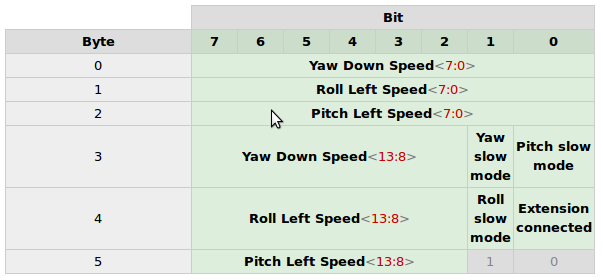
\includegraphics[width=.80\textwidth]{motionPlusDataFormat.png}
    \caption{\footnotesize Motion Plus data gyroscope data format}
    \label{fig:motionPlusDataFormat}
\end{figure}

Motea parsing and calibrating gyroscope data:
\begin{lstlisting}
// Get fast/slow mode
boolean yawFast = ((extensionData[3] & 0x02) >> 1) == 0;
boolean rollFast = ((extensionData[4] & 0x02) >> 1) == 0;
boolean pitchFast = ((extensionData[3] & 0x01) >> 0) == 0;

// Get raw data
float yaw = 
	((extensionData[0] & 0xff) | ((extensionData[3] & 0xfc) << 6));
float roll = 
	((extensionData[1] & 0xff) | ((extensionData[4] & 0xfc) << 6));
float pitch = 
	((extensionData[2] & 0xff) | ((extensionData[5] & 0xfc) << 6));

// Manual calibration
if (!calibration.isFinished()) {
	calibration.addCalibrationData(yaw, roll, pitch);
	if (calibration.isFinished()) {
		calibrationData = calibration.getCalibratedData();
	}
}

// Calibrate raw data
yaw -= calibrationData.getYaw0();
roll -= calibrationData.getRoll0();
pitch -= calibrationData.getPitch0();

// Set scaling
if (yawFast) {
	yaw /= HIGHSPEED_SCALING;
} else {
	yaw /= LOWSPEED_SCALING;
}

if (rollFast) {
	roll /= HIGHSPEED_SCALING;
} else {
	roll /= LOWSPEED_SCALING;
}

if (pitchFast) {
	pitch /= HIGHSPEED_SCALING;
} else {
	pitch /= LOWSPEED_SCALING;
}
\end{lstlisting}

\section{Software Architecture}
In this section contains an explanation and documentation of the various software architectural choices.

The two main focuses when creating the architecture was \emph{modifiability} and \emph{usability}. Modifiability was important to insure the ability to replace the Wii remote with other senors without major changes in the source code. Though the main goal of this project does not include the creation of a complex graphical user interface, usability was still considered a priority for the source code to be reused in future work. 

\subsection{Architectural Patterns}
\subsubsection{Event-driven architecture}
Event-driven architecture is an architectural pattern that focuses on the creation and consumption of events. The event emitters creates new events and pushes them to the event consumers. The event consumers uses the events to produce some reaction. Because the event emitter does not directly speak with the event consumers this pattern makes the different components very loosely coupled.

In our case the event emitters will be the motej and motejx libraries. These classes will handle the connection to the Wii remote and the MotionPlus extension and create events when it receives new date from the Wii remote or its extensions. The event consumers will be the models that change the state in accordance to the received events containing the sensor data. Using this pattern the models are not concerned with the way the event emitters are implemented or what kind of sensors they connect to as long as the events emitted are on the same form.

Fortunatly Motej already implemented the event-driven architecture so there was no need to modify the library in this aspect.

\begin{lstlisting}
//Example of event-driven architecture using 
//java.swing.event.EventListenerList and 
//java.util.EventListener

//Event emittor (parts from the Mote class)
EventListenerList listenerList = new EventListenerList();
...
public void addAcceleromterListener(AcceleromterListener<Mote> listener) {
	listenerList.add(AccelertomerListener.class, listener);
}
...
protected void fireAccelerometerEvent(float x, float y, float z) {
	AccelerometerListener<Mote>[] listeners = listenerList
			.getListeners(AccelerometerListener.class);
	AccelerometerEvent<Mote> evt = 
		new AccelerometerEvent<Mote>(this, x, y, z);
	for (AccelerometerListener<Mote> l : listeners) {
		l.accelerometerChanged(evt);
	}
}

//Interface for the listeners (event consumers)
public interface AccelerometerListener<T> extends EventListener {

	public void accelerometerChanged(AccelerometerEvent<T> evt);

}

//Event consumer - example
public class Example implements AccelerometerListener<Mote> {
	...
	public void acceleromterChanged(AcceleromterEvent<Mote> evt){
		//Events are consumed and handled here
	}
}
\end{lstlisting}

\subsubsection{Model View Controller}
In the model view controller pattern the code is separated into three main components (see figure~\ref{fig:mvc}): model, view and controller. The view handles the graphical user interface and its logic displaying the model to the user. The controller updates the model. The model holds the information or state of the application, which is displayed to the user through the model. This setup gives the users the mental model that they are interacting with the model directly.

\begin{figure}[h!]
  \centering
    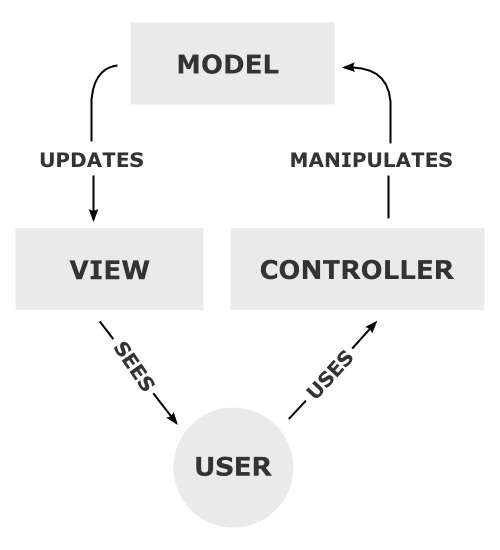
\includegraphics[width=.80\textwidth]{mvc.png}
    \caption{\footnotesize Model-View-Controller pattern}
    \label{fig:mvc}
\end{figure}

Using the model view controller pattern we can easily change the look and feel of the graphical user interface without interfering with how the model is updated. This gives a lot of freedom to continuously modify and improve the graphical user interface during the development of the application. 

\subsection{Package structure}
Using the discussed patterns as a basis, the following package diagram shown in figure~\ref{fig:packageDiagram}. 

\begin{figure}[h!]
  \centering
    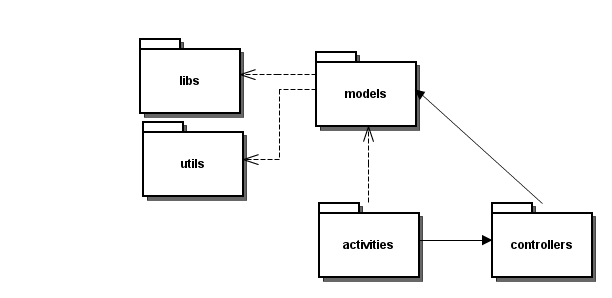
\includegraphics[width=.80\textwidth]{packageDiagram.png}
    \caption{\footnotesize Package diagram}
    \label{fig:packageDiagram}
\end{figure}

\begin{description}
	\item[libs] Contains the library classes used by the project. Currently only contains the java.swing.event.EventListenerList, which is used by Motea. This class is not included in the standard android packages because swing is not part of android.
	\item[utils] The modified Motej library (Modea), our implementation of the MadgwickAHRS algorithm resides here. Motea generates sensor events, and the MadgwickAHRS algorithm is used to calculate orientation.
	\item[models] Classes holding the state of the Wii remote are contained here.
	\item[activities] Holds the Android activity classes. The MainActivity class starts the application and handles Android activity events. The CubeView class is used to generate a 3D-model illustrating the orientation of the connected Wii remote.
	\item[controller] Contains controller classes for interacting with the models and the Wii remote.
\end{description}

\subsection{Activity diagram}
The current application was created to be a proof of concept for the use of Wii remotes in fall detection/prevention applications. Figure~\ref{fig:activityDiagram} displays the basic functionality implemented in the solution. In addition to the 3D model that graphically displays the orientation of the Wii remote, an alarm system was also implemented. This alarm system is activated when the Wii remotes angle is greater than some predefined threshold. This threshold, is as of now, not customizable from the application itself but is hard-coded  into the application for now. 

The alarm uses sound and vibration to notify the user that the Wii remote angle has broken the threshold. Both sound and vibration is given in pulses with a delay between them, as the Wii remote angle becomes grater the delay between each pulse decreases. For the vibrotactile feedback the Wii remote's rumblepack is used and the sound is generated by the Android smartphone speaker. 


\begin{figure}[h!]
  \centering
    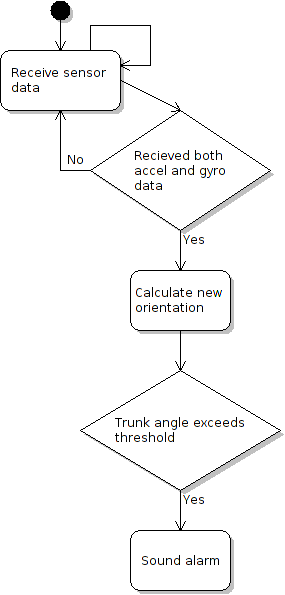
\includegraphics[width=.40\textwidth]{activityDiagram.png}
    \caption{\footnotesize Package diagram}
    \label{fig:activityDiagram}
\end{figure}

\subsection{Class diagram}
Figure~\ref{fig:classDiagram} shows a class diagram of the application's most important classes. The different background colors represents different parts of the system.

The classes with the red background handles the connection to the Wii remote. When the MainActivity class receives a BluetoothDevice object, that object is used to create an instance of Mote. The Mote class connects to the Wii remote. Each second the CheckStatus class is run to get an update about the Wii remote's battery life as well as trying to connect to the MotionPlus, if it is not already connected. The MotionPlus parses the extension bytes received from the Wii remote, it also handles the manual calibration of the gyroscope.

The green background contains the controller classes. WiiMoteHandler handles all communication with the Motea classes (red background). It listens to both the accelerometer and gyroscope events from the Mote instance. When both an acceleromter event and a gyroscope event has been received the WiiMoteHandler WiiRemoteHandlerfires a sensor events. WiiMoteHandler also listens to alarm events to start the rumble pack in the Wii remote when the alarm goes off. Since this class is the only one talking to the Motea classes, this is the only class that needs major changes if it is decided to replace the Wii remotes with other types of sensors. 

AngleCalc listens to sensor events from the WiiMoteHandler, the gyroscope and acceleromter data are used to compute the orientation of the Wii remote and the trunk that it is strapped to. To compute the orientation AngleCalc uses Madgwick's altitude and heading reference system algorithm, which is implemented in the MadgwickAHRS class. AngleCalc then updates the OrientationModel with the newly calculated orientation.

The yellow zone holds the models. OrientationModel hods the current orientation of the Wii remote and then fires an event when it is changed. A very simple noise cancelling system has also been implemented here, to reduce the yaw drift when the Wii remote was kept still. Since the yaw rotation is will not be in the actual fall detection/prevention, this functionality is mainly to make the 3d cube model look better.

ThresholdAlarm listens to orientation events fired by the OrientationModel and then calculates whether the angle of is great enough to fire an alarm event. Alarm events have a severity variable that indicates how great the angle is. In the current implementation this variable is used to reduce the delay between rumble pulses and sound beeps, the greater the angle the faster the beeps.

The views have a blue background. MainAcitivty is the class that starts the application. It also handles Bluetooth discovery and initiates the appropriate classes when a Wii remote is detected. CubeView listens to the orientation evnets from the OrientationModel to crate a graphical representation of the position of the Wii remote. AlarmSound handles playing beeps from the smartphone when the ThresholdAlarm fires alarm events. 

\begin{figure}[h!]
	\centering
	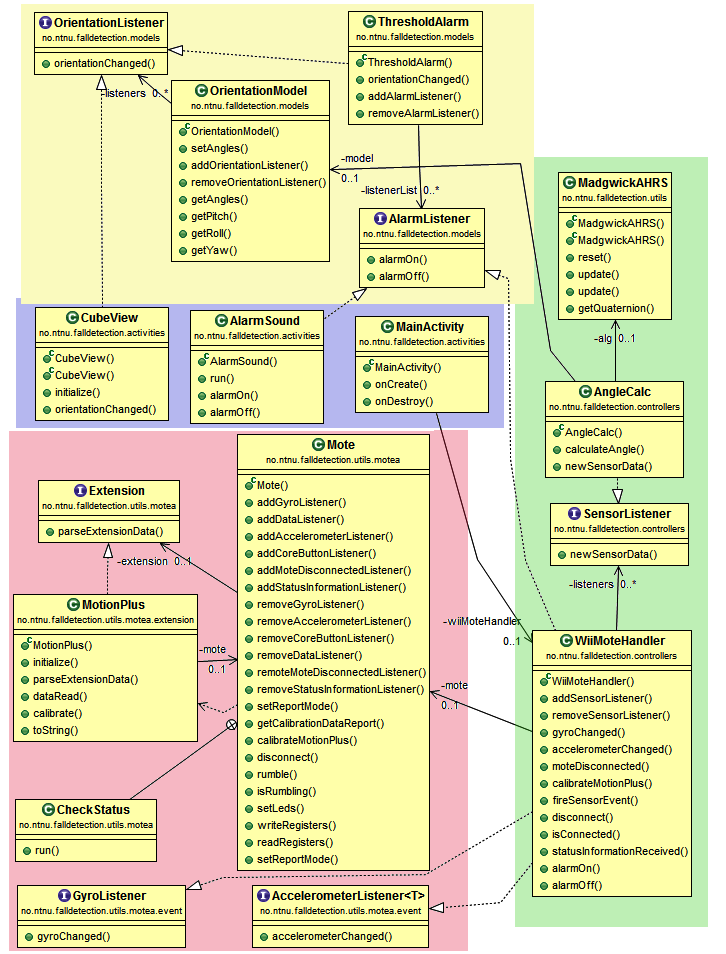
\includegraphics[width=1\textwidth]{classDiagram.png}
	\caption{\footnotesize Class diagram}
	\label{fig:classDiagram}
\end{figure}

\section{Limitations}
%Se på dette avsnittet knut. Tror hele må skriver på nytt hvor avsnittene under er merget og forklart bedre
The majority of Android devices have built-in Bluetooth cards, but the current Android SDK does not offer low level support for the Bluetooth stack, including L2CAP. This constraint can be bypassed on some devices by using reflection to access the socket constructor\cite{l2capHtc}. Access could also be gained through using the Android NDK (Native Developer Kit) but this is outside the scope of this project. Due to L2CAP not being official supported, certain vendors of Android devices have removed the L2CAP protocols completely, meaning that it would be impossible to use their Android OS to connect to the Wii Remote. %Write it more technical
Therefore the Android OS on the HTC Desire HD was altered to run with CyanogenMod 7 instead of the default HTC Sense.

We are unable to connect to new WiiRemote probably due to a different way of initilization.

Have to remove/add the gyroscope in order for the application to register it


\section{Motej and Motejx}
The most complete of the Java based Wii remote libraries that could be found was Motej. Work on the library was discontinued in 2009, but supports all the main Wii remote functionality, and most of the extensions. It was therefore decided to use Motej as the base for a Wii remote library for Android. 

Figure~\ref{fig:motejClassDiagram} shows the most important classes of the Motej and Motejx libraries. To use the library you would create an instance of the Mote object, which takes care of handling the connection to the Wii remote. The Mote constructor takes a string with the bluetooth address of the Wii remote to connect to as input. It is also possible to use the MoteFinder class to discover any Wii remotes that are broadcasting for a connection. The Motej instance fires events whenever it receives data from the Wii remote, these events can be listened to by implementing the different listeners in the motej.events package. 

Wii remote extensions are handled by the Motejx library, which is an extension to the Motej library. All supported extensions have to be added to a extensions.properties file, which contains the extension id and the class that handles that type of extension. This way Motej does not need to know about any of the different extension implementations in the Motejx library, because they all implement the Extension interface. To get data from the Wii remote extensions a listener has to be added to the extension class of that Wii remote extension. So a program wanting to listen to data from the extension has to cast the extension object to the correct extension class in Motejx in order to add listeners.

%Add class diagram of motej and motejx

\section{Motej on Android}
For Motej to work on Android, the BlueCove library has to be replaced with the Android Bluetooth API. This presents a major problem: Wii remotes uses the low level Bluetooth protocol L2CAP to connect to different platforms. As of Android version 4.1, Jelly Bean, \cite{jellyBean} there is no official support for L2CAP. Android only has full support for the higher level protocol \emph{radio frequency communication} (RFCOMM). RFCOMM is built on top of the L2CAP protocol and provides serial port emulation. 

Though the L2CAP is not directly supported through the Android Bluetooth API it is possible to create an L2CAP socket using a technique called reflection.

\begin{lstlisting}
Class<BluetoothSocket> cls = BluetoothSocket.class;
Constructor<BluetoothSocket> constructor = cls.getDeclaredConstructor(
		int.class, int.class, boolean.class, boolean.class,
		BluetoothDevice.class, int.class, ParcelUuid.class);

int type = 3, fd = -1, port = 0x13;
boolean auth = false, encrypt = false;
// Get some device
BluetoothDevice device = getBluetoothDevice();
ParcelUuid uuid = null;

/* type    - Type of socket (3 for L2CAP)
 * fd      - File descriptor (-1 for new socket)
 * auth    - Require authenticaton
 * encrypt - Require encrypted connection
 * port    - Remote port
 * uuid	   - SDP UUID
 */
// This will crate an L2CAP socket on port 0x13
BluetoothSocket socket = constructor.newInstance(type, fd, auth,
		encrypt, device, port, uuid);
\end{lstlisting}

This method has limitations. Because there is no official support for L2CAP in Android, many vendors roms will throw errors when trying to Bluetooth devices this way. Major vendors such as HTC and Samusng does, as of now, not support L2CAP connections.

\section{Motion Plus Support}
Motej has support for most of the common extensions for the Wii remote. Unfortunately Motion Plus is not one of the supported extensions. Motion Plus was implemented using the already existing extension structure of the Motej library.

Information on how to parse the incoming bytes from the Wii Remote was found on the WiiBrew wiki \cite{wiiBrew}. See section~\ref{sec:gyroParse} for a more detailed description of how the data is parsed. 

An additional class was added for manual calibration of the gyroscope. There is calibration data stored in the Wii remote memory, but WiiBrew states that how to use these data for calibration is still unknown. Some suggestions on how to use the data exist, however the calibrated values are not very accurate compared to the manual calibration method. During manual calibration it is required that the Wii remote is kept still. The calibration takes less than 1 second.

\section{Calculating orientation}
%Intro til seksjonen

%Hvorfor trenger vi også akselerometerdata?
%Skrive litt om drift?

%Hvordan funker den, si noe overordnet om smarte ting som quaternions og sånn

A major disadvantage with the Wii Remote compared to competing gaming peripherals such as PS Move and Kinect is that the data output is always relative to itself. In other words, the Wii Remote does not say anything about where it is located in space. Even though the Wii Remote does not provide its orientation out of the box, the data it does provide is enough for developers to calculate the orientation of the Wii Remote. Calculating the orentation of the Wii requires dedicated algorithms that used advanced mathematical formulas. Calculations are performed on the sensor data collected from the Wii Remote and Motion Plus extension. The accelerometer data enables developers to determine the tilt of the Wii Remote while gyroscope data allows developers to determine the movement speed in three directions. Only by utilizing both can the algorithms calculate the orientation of the Wii Remote.

We chose to use the Madgwick algorithm\cite{madgwick}. This choice was based on the fact that a master thesis by Tryggestad\cite{Tryggestad} had used the same algorithm for Wii Remote orientation successfully. A C\# implementation of the algorithm is available at the x-io Technologies Limited website \cite{opensourceMadgwick}, we used this as a basis for the Java implementation of the algorithm which is used in our application. The constructor of the algorithm requires two parameters a sample periode and an algorithm gain beta. The sample period was set to 1f/100f and the algorithm gain beta was set to 0,5f. Sample periode is equal to the refresh rate of the Wii Remote and the beta is based on findings by Tryggestad. These values proved to be satisfactory for us as well.

\begin{figure}[h!]
  \centering
    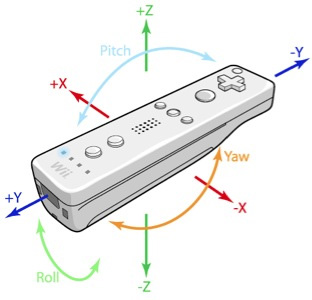
\includegraphics[width=.45\textwidth]{wiimoteAxis.png}
    \caption{\footnotesize A visual representation of the cartesian coordinate system for the Wii Remote, taken from Wii Brew\cite{wiiBrew}.}
\end{figure}

% Sette algoritmen i appendix?

The algorithm update method requires six parameters: The first three are the gyroscope's X, Y, and Z axis measurements provided in radians/, the following three are the accelerometers X Y Z in any calibrated unit. We discovered that what is defined as yaw, pitch, and roll is not universal, and which axis each corresponds to might be different for aviation and gaming controllers. Rotation about the X axis corresponds pitch, Y corresponds roll and Z corresponds to yaw such as shown in % REF TO IMAGE %WRITE MORE ABOUT HOW IT WORKS WITH ACCEL/GYRO
The algorithm returns the result as a Quaternion that need to be stored and converted to Euler angles. The formulas for converting the Quaternion to Euler angles are provided in the Madgwick paper. The formula for roll is incorrect in the paper, providing us with incorrect values, Tryggestads calculation was used for the roll conversion. The change was minor as Madgwick uses the wrong quaternion unit for roll calculation.

%SHINY PICTURZS OF OUR CODE

\section{Motea}
\label{sec:motea}
During the modification of the Motej library it soon became apparent that several parts of the library were outdated or not optimal for the current application. One problem was discovered when implementing rumbling response to alarm events. The rumble pack was turned off each time a request for status information was sent to the Wii remote. This bug was caused by the fact that Motej did not modify the status information request with the current status of the rumble pack.

It was also discovered that Motej used an outdated port to send requests to the Wii remote. Motej used the control pipe with report 0x52 to send requests. This method only works for the original Wii remotes, and will not work for the newer models. During testing the original Wii remote with external MotionPlus was used and therefore this problem was not discovered before later in the development phase.

Because of all the small bugs and the large portions of the library that were not used it was decided to create a lightweight Wii remote library from scratch. The new library was based on the general structure of Motej, and some of the code was also reused. Motea uses the data pipe for both sending and receiving data from the Wii remote. This way the new library should suppor the newer Wii remotes. 

Currently these input report modes are supported:
\begin{description}
	\item[0x20] Status information
	\item[0x21] Read memory and registers
	\item[0x37] Core buttons, acceleromter, extension data (gyroscope)
\end{description}

Report mode 0x37 also contains bytes with data from the IR camera, but this functionality was not needed and therefore not added to the Motea library.

Supported output reports are:
\begin{description}
	\item[0x11] Set LEDs and activate rumble pack
	\item[0x12] Sed data report mode (only 0x37 will be used)
	\item[0x15] Status information request
	\item[0x16] Write to memory and registers (used for activating MotionPlus)
	\item[0x17] Read memory and registers (for calibration reports)
\end{description}

The new library has working support for rumbling and connecting the MotionPlus extension while rumbling, which also was problematic with Motej. Motea also sends requests for status information and checks for MotionPlus (if not connected) each second. This way any class listening to status information events get regular updates, and not just when an extension is connected.

\section{Prototype application}
The graphical user interface of the application is quite simplistic, there are two reasons for this. The first being that this prototype is more focused on the technology and viability of a bio-feedback system based on a Wii Remote and an Android device, then the user interface. The application is intended those who do not have great coordination or muscle control, so we are trying to keep the interaction with the phone to a minimum, and when they do need to interact with it, then it should be easy and very simple.

The GUI consists of 3 components, two buttons and a visual representation of the Wii Remote. A connection with the Wii Remote is attained by pressing the (1) and (2) buttons on the Wii Remote, and afterwards pressing the "Connect" button on the application. The button will change from "Connect" to "Connecting.." in order to inform the user that it is attempting to establish a connection. Once a connection has been established the "Connect" button will be grayed out an changed to "Connected". A connection is confirmed by the 3D box coming to life, and any movement of the Wii Remote is mirrored by the box on screen. A successful connection will also be indicated on the Wii Remote due to the LEDs on the controller being lit. The LEDs represent the battery life; All four LEDs lit means that the Wii Remote battery is full.

PICTURE OF APPLICATION

Once a successful connection has been established the Wii Remote should be calibrated in order to achieve optimal accuracy. Through the use of the gyro data the Madgwick algorithm is able to correct inaccurate data. The WiiMote does contain calibration constants sadly these are not accurate. A gyro velocity of up to 30 rad/s is reported when the WiiMote is in fact standing still. Through manual calibration this error is reduced to approximately 0. Calibration is achieved by placing the Wii Remote in the desired position and then pressing the "Calibrate" button.

The position of the WiiMote at the time of calibration will be set as the starting point when calculating angular displacement. Once the angular displacement is above the set threshold a beep sound will be activated in set internvals, and the WiiMote will vibrate in tune with the beeps. The frequency of the vibration and beeps will increase as the angular displacement increases, and 90 degrees being the max intensity.
